%!TEX root = ../terrainbook.tex
% chktex-file 46

% \setchapterpreamble[u]{\margintoc \marginnote{\faYoutube\ https://3d.bk.tudelft.nl}}
% TODO : youtube link?
\setchapterpreamble[u]{\margintoc}
% \setchapterpreamble[u]{\marginnote{\faYoutube\ https://3d.bk.tudelft.nl}}

\chapter{Handling and processing massive terrains}%
\label{chap:massive}


\graphicspath{{massive/}}


In this chapter we discuss three methods to handle and/or process {\LARGE massive} terrains and point cloud datasets.

%

``Massive'' is a vague and undefined term in GIS, and it is continuously changing: 15 years ago a point cloud dataset containing 5 million elevation points was considered massive, but in 2021 it is considered a small one.%
\index{massive datasets}
Examples of massive datasets: 
\begin{enumerate}
  \item the point cloud dataset of a \SI{1.5}{km^2} of Dublin\sidenote{\url{https://bit.ly/32GXiFq}} contains around 1.4 billion points (density of \SI{300}{pts/m^2}), which was collected with airborne laser scanners; 
  \item the lidar dataset of the whole of the Netherlands (called AHN\sidenote{\emph{Actueel Hoogtebestand Nederland} (in Dutch): \url{http://www.ahn.nl}}) has about \SI{10}{pts/m^2} and its latest version (AHN3) has more than 700 billion points (AHN4 will contain even more points);
  \item the global digital surface model \emph{ALOS World 3D---30m (AW3D30)}\sidenote{\url{https://www.eorc.jaxa.jp/ALOS/en/aw3d30/index.htm}} is a raster dataset with a resolution of \ang{;;1}. Thus we have about \num{8.4d11} pixels.
\end{enumerate}

%

We define as ``massive'' a dataset that does not fit into the main memory of a standard computer, which is these days usually around 16GB\@.
This definition makes practical sense because working with data outside of the main memory of a computer is substantially slower (about 2 orders of magnitude for solid state drives and 5 for spinning hard drives), causing many standard data processing algorithms to become impractical with massive datasets.
Keep in mind that not only the $xyz$ coordinates of the points of a point cloud need to be stored, but also often attributes for each point (LAS has several standard ones).
Also, in the case of TINs, the geometry of the triangles---and potentially the topological relationships between them---need to be explicitly stored.

%

What is ironic is that while datasets like those above are being collected in several countries, in practice they are seldom used since the tools that practitioners have, and are used to, usually cannot handle such massive datasets. 
Indeed, the traditional GISs and terrain modelling tools are limited by the main memory of computers: if a dataset is bigger then operations will be very slow, and will most likely not finish (and thus crash).

%

This chapter discusses one method to visualise massive raster terrains, one to index point clouds (for fast retrieval of neighbours, useful for several processing of points), and one to construct massive Delaunay triangulations (and potentially process them).



%%%%%%%%%%%%%%%%%%%%
%
\section{Raster pyramids}%
\index{raster pyramid}

Raster pyramids are a well-known, standardised, and widely used mechanism to deal with large raster terrains.
They are also used for standard images in photography and many software support them since they optimise visualisation and thus the speed of a software dealing with large images (they are called ``tiled pyramidal images'' or ``overview images'').

As shown in \reffig{fig:pyramids}, 
\begin{figure}
  \centering
  \begin{subfigure}[b]{0.65\linewidth}
    \centering
    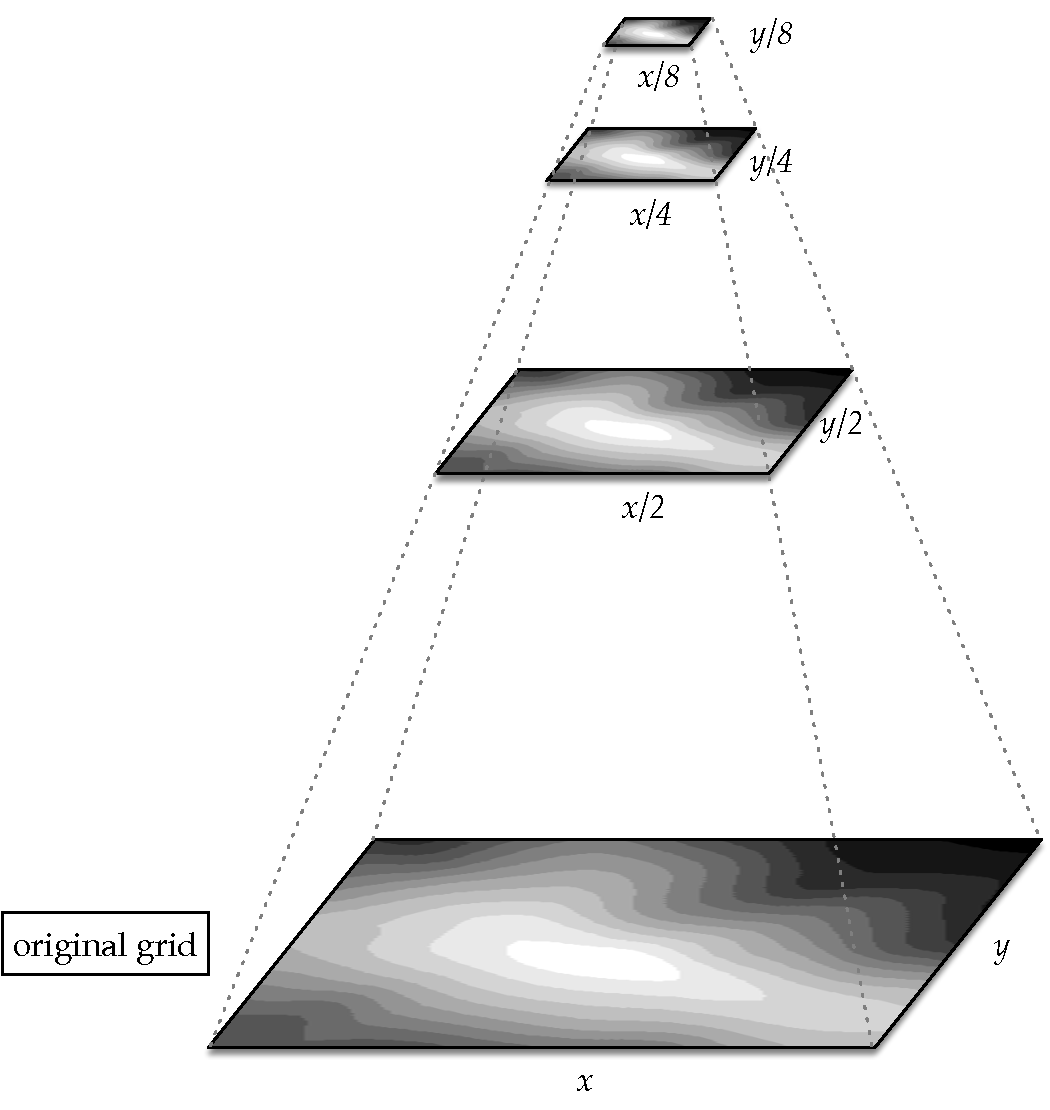
\includegraphics[width=\textwidth]{figs/pyramids.pdf}
    \caption{}
  \end{subfigure}
  \qquad%
  \begin{subfigure}[b]{0.2\linewidth}
    \centering
    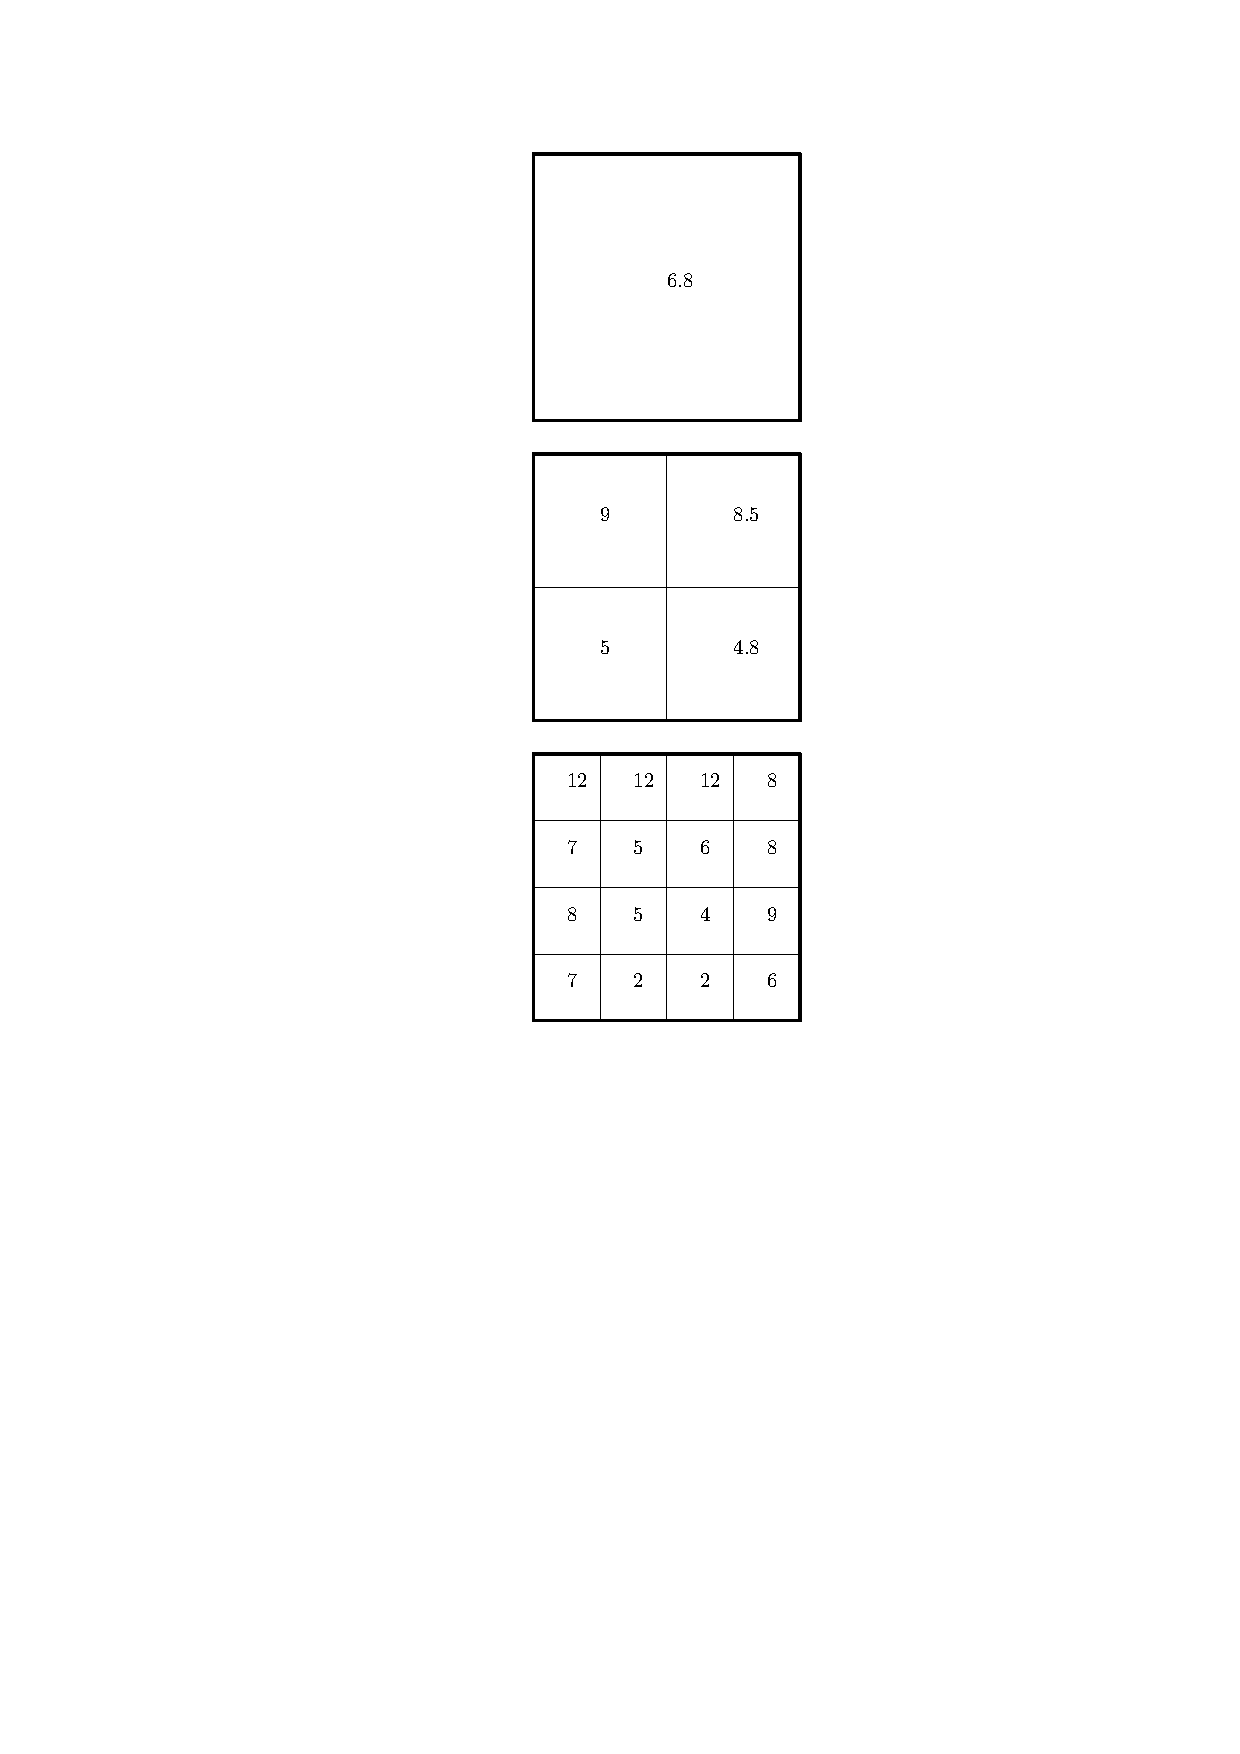
\includegraphics[width=\textwidth]{figs/pyramids2.pdf}
    \caption{}
  \end{subfigure}
\caption{\textbf{(a)} The pyramid for a given raster file. \textbf{(b)} One $4\times4$ raster downsampled twice with average-method.}%
\labfig{fig:pyramids}
\end{figure}
a pyramid means creating recursively copies at lower-resolutions of an original raster.
Usually we downsample the resolution by a factor 2,% 
\index{downsampling}\marginnote{downsampling}
\ie\ if we have $x$ columns and $y$ rows the first copy will have a size ($\frac{x}{2}$, $\frac{y}{2}$), the second ($\frac{x}{4}$, $\frac{y}{4}$), and so on (the number of images is arbitrary and defined by the user).
Notice that the extra storage will be maximum $\frac{1}{3}$ of the original raster: the first pyramid is $\frac{1}{4}$, the second $\frac{1}{16}$, the third $\frac{1}{64}$, etc.

%

For downsampling, the most common method is based on averaging the 4 pixel values that are merged into one (as shown in \reffig{fig:pyramids}b), but other interpolation methods are possible, \eg\ nearest neighbour as seen in \refchap{chap:interpol}.

%

The downsamples grids are used to speed up visualisation (when a user zooms out on a lower-resolution grid is displayed) but the same principle could be applied to for processing (\eg\ the line-of-sight between 2 points in Chapter~\ref{chap:visibility} could be sped up by using this principle).

\begin{floatbox}
\begin{kaobox-practice}[frametitle=\faCog\ How does it work in practice?]
  For certain GIS formats, \eg\ GeoTIFF, the lower-resolutions rasters can be stored directly in the same file as the original raster, and this is standardised.

  For other formats, if the GDAL library is used (the \emph{de facto} open-source library for GIS images and grids), the pyramids can be stored in an auxiliary file with the extension \texttt{.ovr}, which is actually a TIFF format.

  The GDAL utility \href{https://www.gdal.org/gdaladdo.html}{gdaladdo \faExternalLink} can create automatically the pyramids for a few formats, and the downsampling method can be chosen.
  In QGIS, one can use \texttt{gdaladdo}, or there is also a built-in mechanism, as can be seen in \reffig{fig:qgis}
\end{kaobox-practice}
\end{floatbox}

\begin{figure}
  \centering
  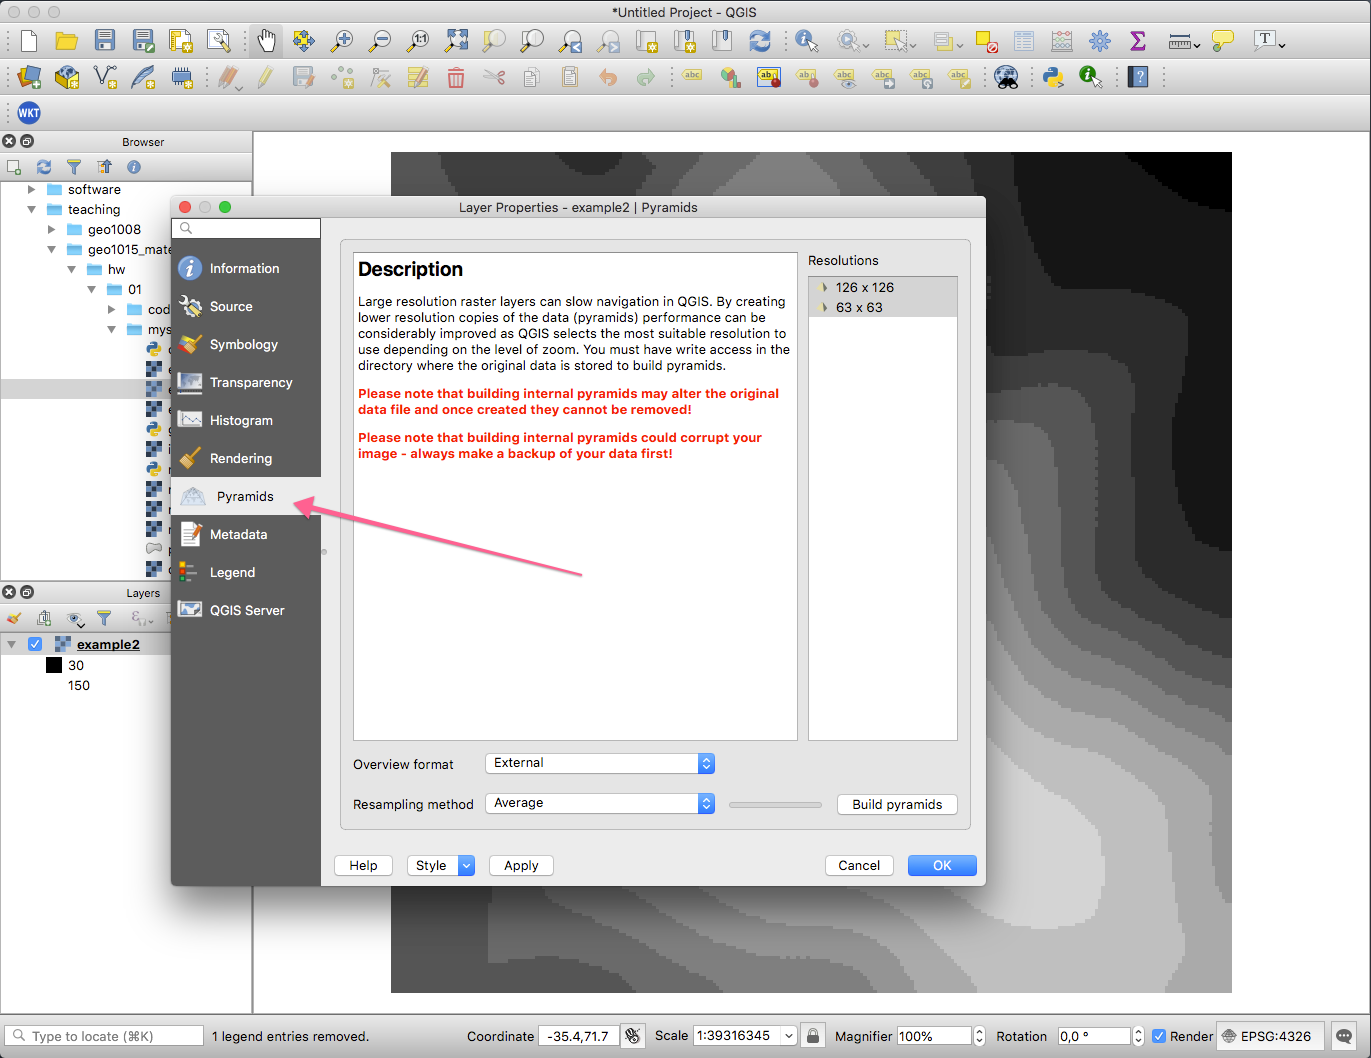
\includegraphics[width=\linewidth]{figs/qgis}
  \caption{QGIS has the option to create the pyramids automatically.}%
\labfig{fig:qgis}%
\end{figure}



%%%%%%%%%%%%%%%%%%%%
%
\section[kd-tree]{Indexing points in 3D space with the kd-tree}%
\label{sec:kdtree}\index{kd-tree}

\begin{marginfigure}
  \centering
  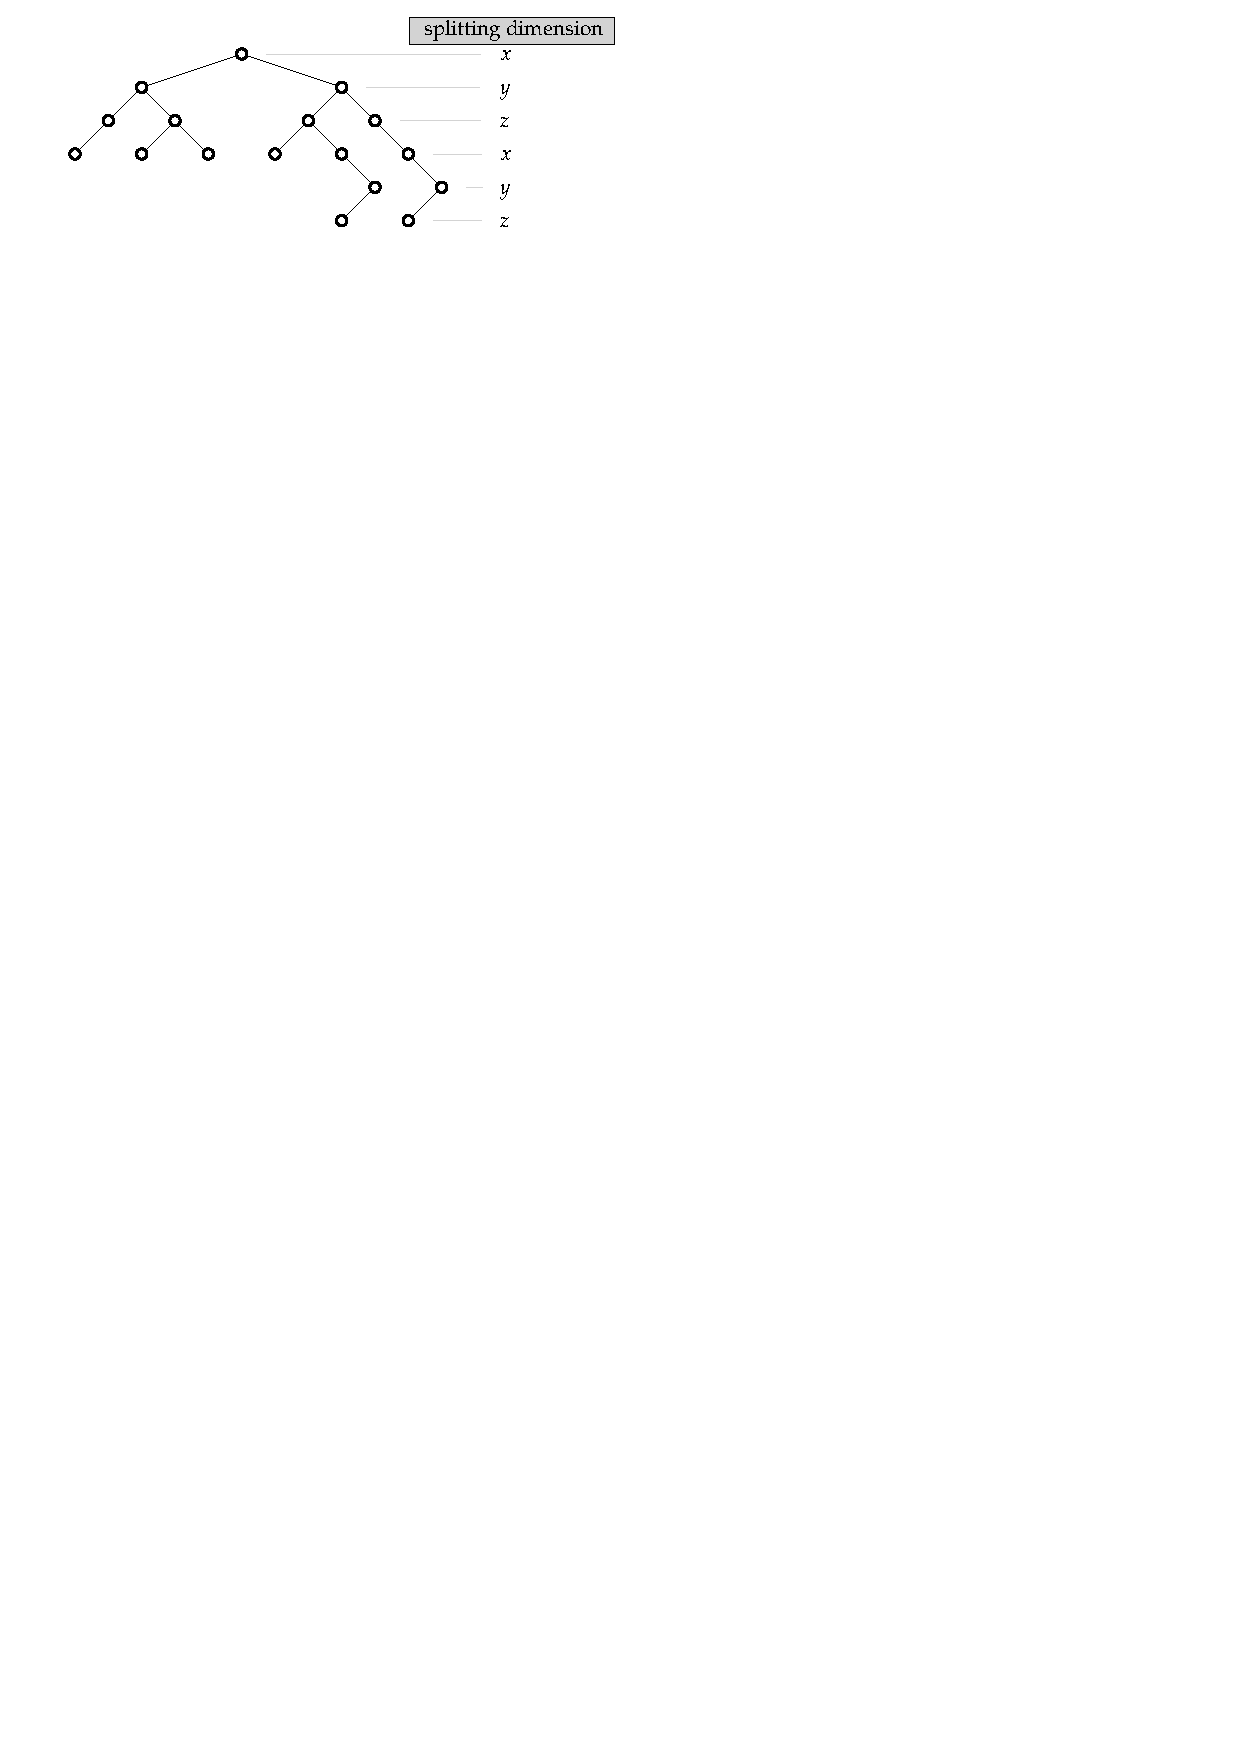
\includegraphics[width=\linewidth]{figs/kdtree}
  \caption{Example of $k$d-tree in 3D, with the dimension used at each level.}%
\labfig{fig:kdtree}
\end{marginfigure} 

A $k$-dimensional tree, $k$d-tree in short, is a data structure to organise points in a $k$-dimensional space; it also partitions the space into regions.
In the context of terrains, $k$ is in most cases either 2 or 3.
Notice that in practice we would never say a ``2d-tree'' or a ``3d-tree'': we call them ``$k$d-tree of dimension 2 (or 3)''.

%

As shown in \reffig{fig:kdtree}, a $k$d-tree is a binary tree%
\index{binary tree}\marginnote{binary tree}
(thus each node has a maximum of 2 children, if any), and the main idea is that each level of the tree compares against one specific dimension.
We `cycle through' the dimensions as we walk down the levels of the tree.

%

Let $S$ be a set of points in $\mathbb{R}^k$, and let $\Gamma$ be the $k$d-tree of dimension $k$ of $S$.
Each point $p_i$ in $S$ is a node of $\Gamma$.
A node implies a hyperplane% 
\index{hyperplane}\marginnote{hyperplane}
that divides the space into 2 halfspaces according to one dimension; the hyperplane is perpendicular to the dimension of the node (which is linked to the level in the tree).
Points with a lower coordinate value than the node along that dimension (corresponding to `left', in 2D, or `under' the hyperplane) are put into the left subtree of the node, and the other ones into the right subtree.

Consider the $k$d-tree in 2D in \reffig{fig:kdtree2}.
\begin{figure}[tbp]
  \centering
  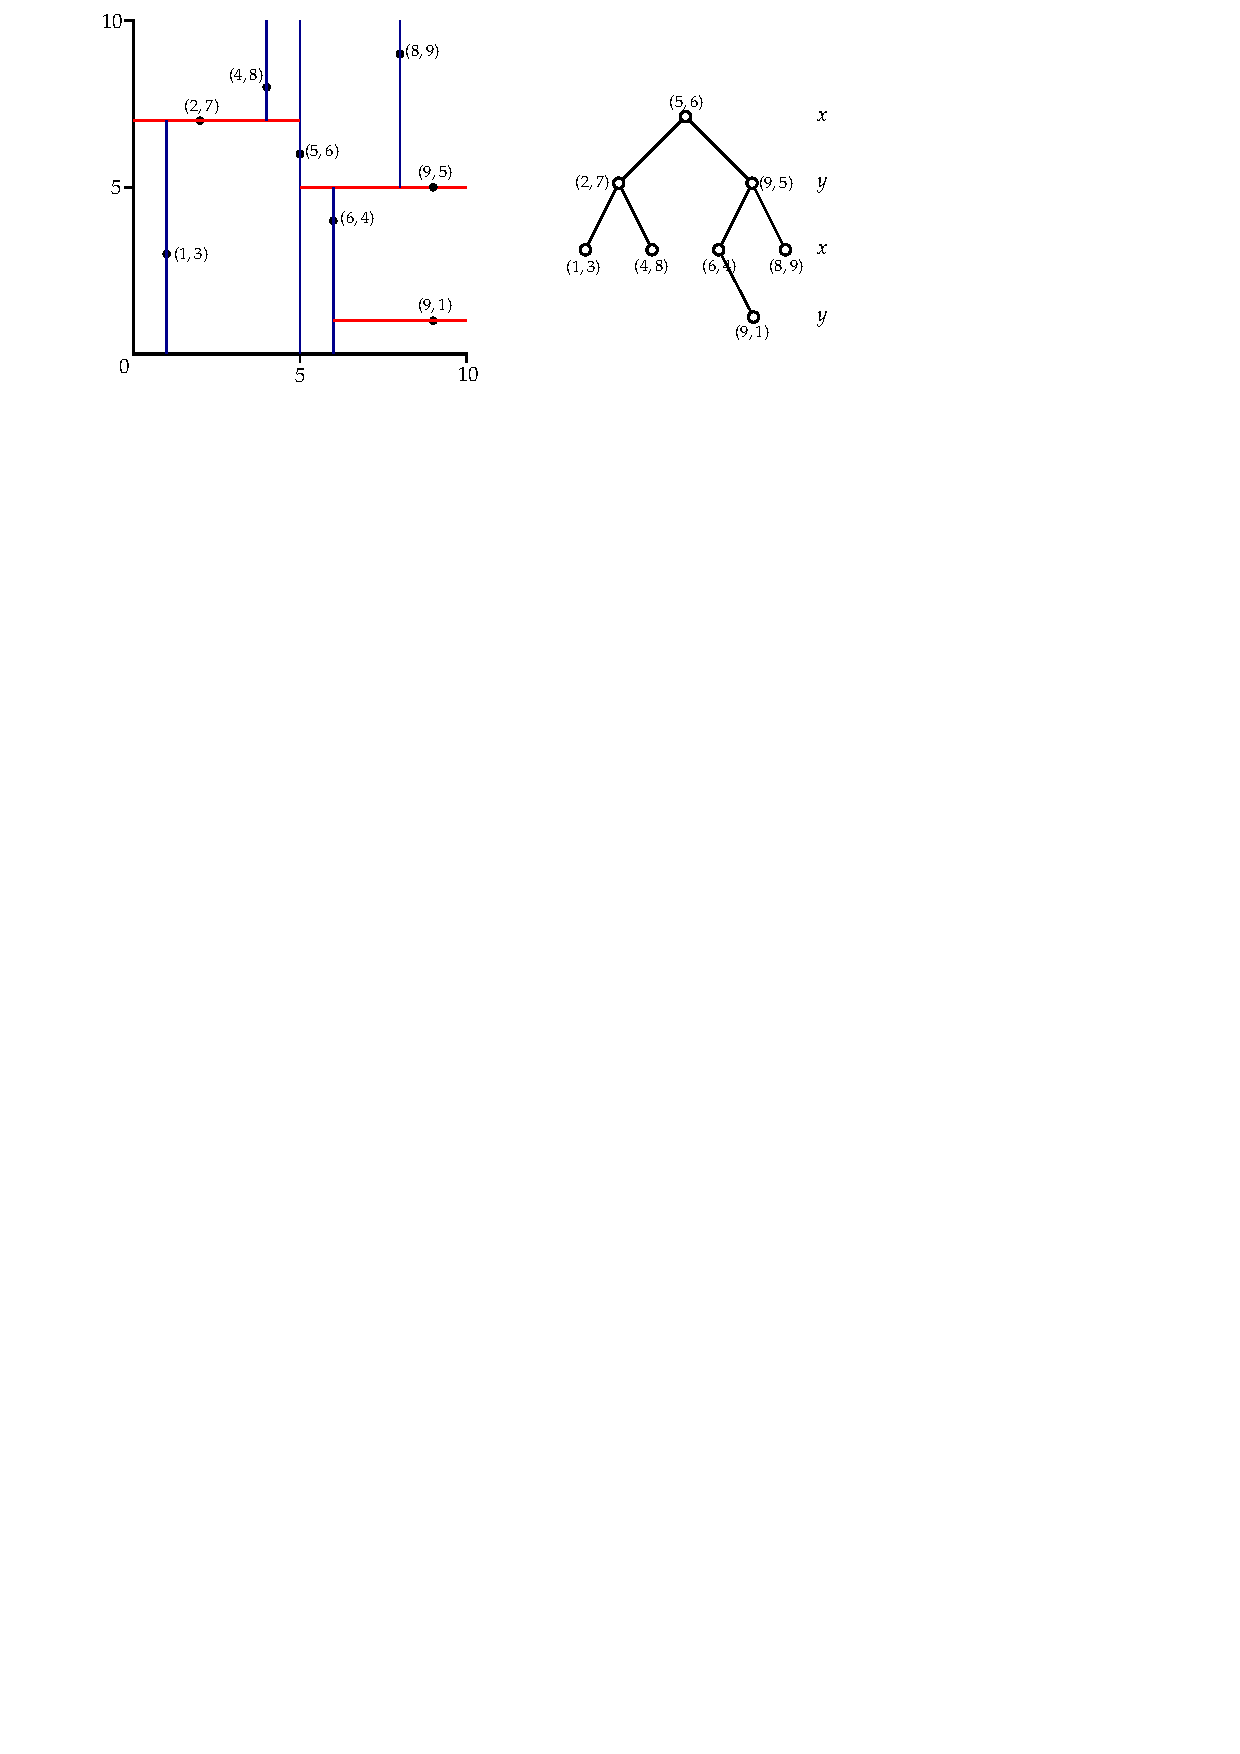
\includegraphics[width=0.9\linewidth]{figs/kdtree2}
  \caption{Example of $k$d-tree for 8 points in the $\mathbb{R}^2$.}%
\labfig{fig:kdtree2}
\end{figure}
The first dimension splits the data into 2 halfplanes along the line $x=5$, then each of these halfplanes is independently split according to the $y$ dimension (with the lines $y=7$ and $y=5$), then the 4 regions are split according to the $x$ dimension, and so on recursively until all the points in $S$ are inserted in $\Gamma$.

%%%
\paragraph{Construction of a kd-tree.}
In theory, any point could be used to divide the space according to each dimension, and that would yield a valid $k$d-tree.
However, selecting the \emph{median} point creates a \emph{balanced} binary tree,%
\marginnote{selecting the median creates a balanced tree} 
which is desirable because it will improve searching and visiting the tree (see below).
The tree in \reffig{fig:kdtree2} is balanced, but if for instance ($1,3$) had been selected as the root, then there would be no children on the left, and all of them would be on the right.

The median point is the one whose value for the splitting dimension is the median of all the points involved in the operation.
This implies that to construct the $k$d-tree of a set $S$ of $n$ points, as a first step $n$ values need to be sorted, which is a rather slow operation ($\mathcal{O}(n \log n)$).
In practice, most software libraries will not sort $n$ values, but rather sample randomly a subset of them (say 1\%), and then use the median of this subset as the splitting node in the graph.
While this does not guarantee a balanced tree, in practice the tree should be close to balanced.

The tree is built incrementally, \ie\ points are added in the tree one after the other, and after each insertion the tree is updated.
Each insertion is simple: traverse the tree starting from the root, go left or right depending on the splitting dimension value, and insert the new point as a new leaf in the tree.
\reffig{fig:kdtree_insert}
\begin{figure}[tbp]
  \centering
  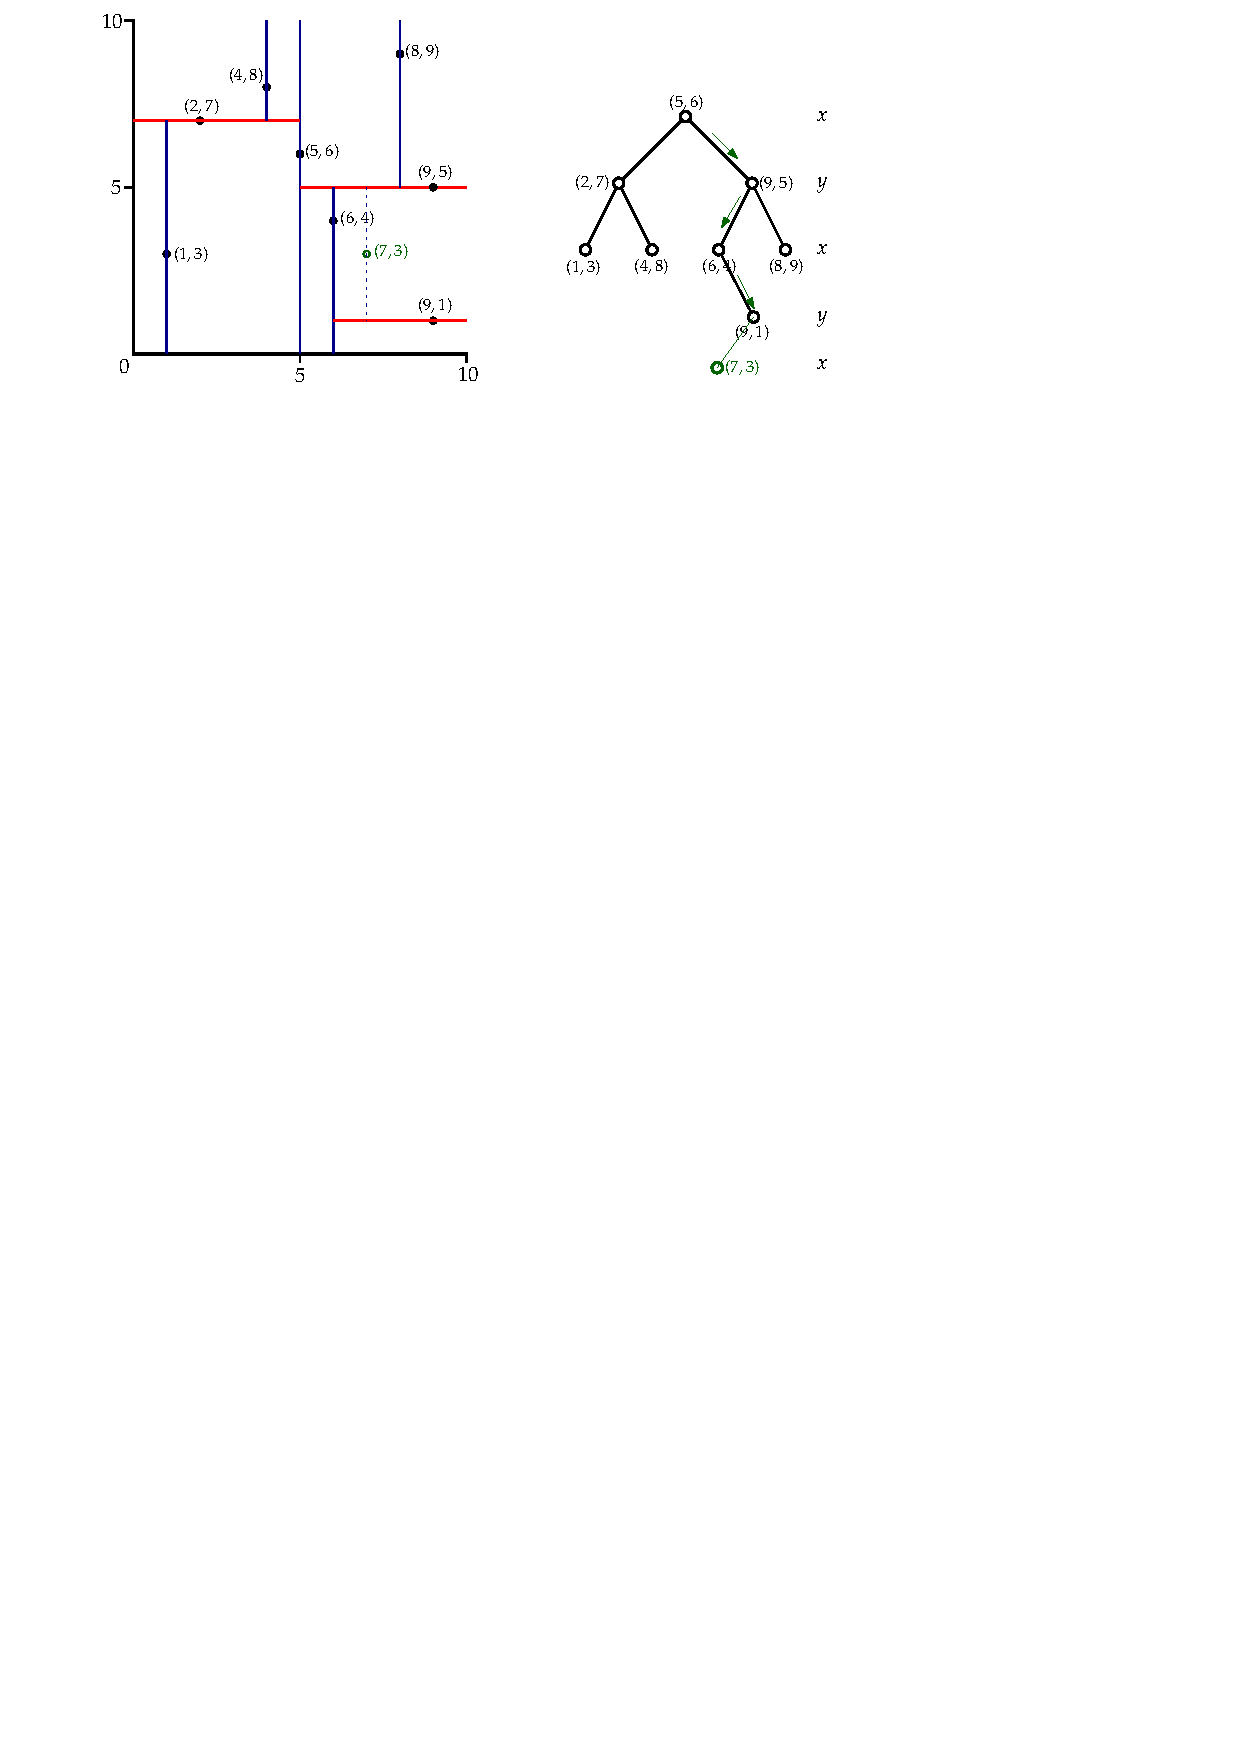
\includegraphics[width=0.9\linewidth]{figs/kdtree_insert}
  \caption{Insertion of a new point ($7,3$) in a $k$d-tree.}%
\labfig{fig:kdtree_insert}
\end{figure} 
illustrates this for one point.

Observe that this insertion renders the tree unbalanced.
Methods to balance a $k$d-tree exists but are out of scope for this book.


%%%
\paragraph{Nearest neighbour query in kd-trees.}%
\label{sec:knn}

The nearest neighbour query%
\index{nearest neighbour query}\marginnote{nearest neighbour query}
aims to find the point $c$ in a set $S$ that is the nearest (according to the Euclidean distance) to a query point $q$.
It can be performed brute-force (computing all the distances to all the points in $S$ and choosing the shortest), but this is very slow in practice.
An alternative is to construct the Voronoi diagram (or the Delaunay triangulation), and navigate in the cells or in the triangles with the method from Section~\ref{sec:dtwalk}.
While this works, in practice it is not as efficient as using a $k$d-tree.

% We discuss here what a $k$d-tree, how to construct one, and how it can be used to efficiently find the nearest neighbour(s) of a query point $q$.

%

First observe that the obvious method to find the cell in the $k$d-tree containing $q$---follow the insertion steps as described above and look for the parents---does not work because $q$ can be far away in the tree.
\reffig{fig:kdtree_nn}a illustrates this: $c$ (the nearest neighbour to $q$) is ($6,4$) but is located in the right subtree of the root, while $q$ is in the left subtree.
\begin{figure*}
  \centering
  \begin{subfigure}[b]{0.6\linewidth}
    \centering
    \includegraphics[page=2,width=\textwidth]{figs/kdtree_nn.pdf}
    \caption{}
  \end{subfigure}
  \begin{subfigure}[b]{0.6\linewidth}
    \centering
    \includegraphics[page=3,width=\textwidth]{figs/kdtree_nn.pdf}
    \caption{}
  \end{subfigure}
  \begin{subfigure}[b]{0.6\linewidth}
    \centering
    \includegraphics[page=4,width=\textwidth]{figs/kdtree_nn.pdf}
    \caption{}
  \end{subfigure}
  \begin{subfigure}[b]{0.6\linewidth}
    \centering
    \includegraphics[page=5,width=\textwidth]{figs/kdtree_nn.pdf}
    \caption{}
  \end{subfigure}
\caption{Several states for the nearest neighbour query based on a $k$d-tree, $q=(4.5, 4.0)$ is the query point and $c=(6,4)$ is the nearest point.}%
\labfig{fig:kdtree_nn}
\end{figure*}


%

The idea of the algorithm we are presenting here is to traverse the whole tree (in depth-first order), but use the properties of the tree to quickly eliminate large portions of the tree.
The eliminated subtrees are based on their bounding boxes.
\marginnote{subtrees are eliminated based on their bounding boxes}
As we traverse the tree, we must keep track of the closest point $c_{temp}$ so far visited.

% and the observation that they cannot contain any point closer

The algorithm starts at the root, stores the current closest point $c_{temp}$ as the root, and visits the nodes in the tree in the same order as for the insertion of a new point.
This order is the one that is \emph{most promising}, because we expect $c$ to be close to the insertion location (albeit this is not always the case).
At each node $n_i$ it updates $c_{temp}$ if it is closer.
For this, the Euclidean distance is used.
For the example in \reffig{fig:kdtree_nn}b, point ($5,6$) is the first $c_{temp}$, and then although ($2,7$) and ($1,3$) are visited, neither is closer and thus after that step $c_{temp} = (5,6)$.

The algorithm then recursively visits the other subtrees, and checks whether there could be any points, on the other side of the splitting hyperplane, that are closer to $q$ than $c_{temp}$.
The idea behind this step is that most of the subtrees can be eliminated by verifying whether the region of the bounding box of the subtree is closer than the current $dist(q, c_{temp})$, $dist()$ being the Euclidean distance between 2 points.
If that distance is shorter, then it is possible that one point in the subtree is closer than $c_{temp}$, and thus that subtree must be visited. 
If not, then the whole subtree can be skipped, and the algorithm continues.

\reffig{fig:kdtree_nn}c shows this idea after ($1,3$) has been visited.
$c_{temp}$ is ($5,6$), and we must decide whether the subtree right of ($2,7$) must be visited.
In this case it must not be visited because the bounding box (light blue region) is 3.0unit from $q$, and $dist(q,c_{temp})$ is around 2.07; it is thus impossible that one point inside the subtree be closer than ($5,6$).

The next step is verifying whether the subtree right of the root could contain a point closer than $c_{temp}$.
In the \reffig{fig:kdtree_nn}d, this is possible since the bounding box is only 0.5unit from $q$, and thus the subtree must be visited.

The algorithm continues until all subtrees have either been visited or eliminated.
At the end, $c$ is ($6,4$).


\paragraph{Time complexity.}
To insert a new point, and to search for a nearest neighbour, the time complexity on average is $\mathcal{O}(\log n)$; this is assuming the tree is balanced, if not it could be $\mathcal{O}(n)$ in the worst-case.
The tree stores one node per point, thus the space complexity is $\mathcal{O}(n)$.

\paragraph{$m$-closest neighbours.}
% from Wiki
The algorithm can be extended in several ways by simple modifications. 
It can provide the $m$ nearest neighbours to a point by maintaining $m$ current closest points instead of just one. 
A branch is only eliminated when $m$ points have been found and the branch cannot have points closer than any of the $m$ current bests. 
This can help improve significantly the running time of several operations described in this book: IDW with a fixed number of neighbours (Section~\ref{sec:wam_interpol}), extracting shapes from point clouds (Section~\ref{sec:shape-detection}), calculating the spatial extent (Chapter~\ref{chap:spatialextent}), are only but a few examples.

% \begin{kaobox-practice}[frametitle=\faCog\ How does it work in practice?]
% python the easiest is ckdtree from scipy
% astest I know is this: https://github.com/storpipfugl/pykdtree
% \end{kaobox-practice}

%%%%%%%%%%%%%%%%%%%%
%
\section[Streaming paradigm]{Streaming paradigm to construct massive TINs and grids from point clouds}%
\label{sec:streaming}

The incremental construction algorithm for the Delaunay triangulation (DT), presented in \refchap{chap:dtvd}, will not work if the size of the input dataset is larger than the main memory.
Or if it works, it will be very slow.
The reason for this is that the data structure for the DT (to store the points coordinates, and also the data structure for the triangles and their topological relationships) will be partly in the main memory (say 16GB of RAM) and the rest will be on the harddrive, and a part of the data structure is necessary \emph{swapping}% 
\marginnote{swapping and trashing}
between the memory and the disk will be performed, and it is possible that if a lot (too many operations) of swapping are performed the process stops (called \emph{trashing}).

%

One solution to this problem, is to design external memory algorithms.%
\index{external memory algorithms}\marginnote{external memory algorithms}
These basically do not rely on the operating system to decide which parts of the data structure are stored on the disk, but improve the process by explicitly storing temporarily files and having explicit rules for the swapping of data between the disk and the memory. 
% \citet{Agarwal05} construct massive TINs this way, and \citet{Arge06} and \citet{Agarwal08} have implemented spatial analysis functions on TINs based on that paradigm.
The main drawbacks of this approach are that the design of such algorithms is rather complex, that for different problems different solutions have to be designed, and that for problems like the DT construction a lot of large temporary files need to be created.

%

We present in this section an alternative approach to dealing with massive datasets: \emph{streaming}.%
\index{streaming data}\marginnote{streaming data} 
The streaming paradigm means here that large files can be process without them to be fully loaded in memory (or that the algorithm has a global access to the said file).
One concrete example is YouTube: to watch a given video one does not need to first download the whole file, they can simply start watching the video as soon as the first KB are downloaded.
The content of the video is downloaded as one watches the video, and if the user fast-forward to for instance 5:32s then only the KB of content from where the cursor is need to be downloaded.
At no moment is the full video downloaded to the user's device.

%

This idea can be used to process geometries (points, meshes, polygons, etc.) but it is slightly more involved than for a simple video.
Since the First Law of Geography of Tobler stipulates that ``everything is related to everything else, but near things are more related than distant things''\marginnote{Tobler W., (1970) \emph{A computer movie simulating urban growth in the Detroit region}. Economic Geography, 46(Supplement):234–240}, if we wanted to calcute the slope of at one location in a point cloud we would need to retrieve all the neighbours and we saw above that this can be done with a kd-tree.
The question is: is it possible to do this without reading the whole file and only process one part of it?

%

We focus in the following on the creation of a DT\@.
The issue that we are facing is that a triangle is respecting the Delaunay criterion if its circumcircle is empty of any point, therefore while constructing the DT we need to test all the other points in the dataset to ensure that a given triangle is Delaunay (or not).
Streaming would mean here: can we assess that a given triangle is Delaunay without having to read/download the whole file?

\begin{floatbox}
\begin{kaobox-practice}[frametitle=\faCog\ Streaming is realised with Unix pipes]
  The key to implementing streaming of geometries is to use Unix pipes (also called \emph{pipelines}).

  Pipelines were designed by Douglas McIlroy at Bell Labs during the development of Unix, and they allow to chain several processes together. The output of a process becomes the input of the next one, and so on (the data flowing through the process is the \emph{stream}). Given 2 processes, the 2nd one can usually start before the 1st one has finished processing all the data.

  In Unix, the pipe operator is the vertical line ``\texttt{|}'', and several commands can be chained with it: ``\texttt{cmd1 | cmd2 | cmd3}''. 
  A simple example would be ``\texttt{ls -l | grep json | wc -l}'' which would:
  \begin{enumerate}
    \item list all the files in the current directory (one file name per line); 
    \item send this to the operator \emph{grep} which would discard all lines not having the keyworld `json'; 
    \item send this to the operator \texttt{wc -l} which counts the number of line.
   \end{enumerate} 
\end{kaobox-practice}
\end{floatbox}

%%%
\paragraph{Overview of streaming DT construction.}
Figure~\ref{fig:streamingdt} shows the overview of the processes involved for the construction of a DT with the streaming paradigm.
\begin{figure}
  \centering
  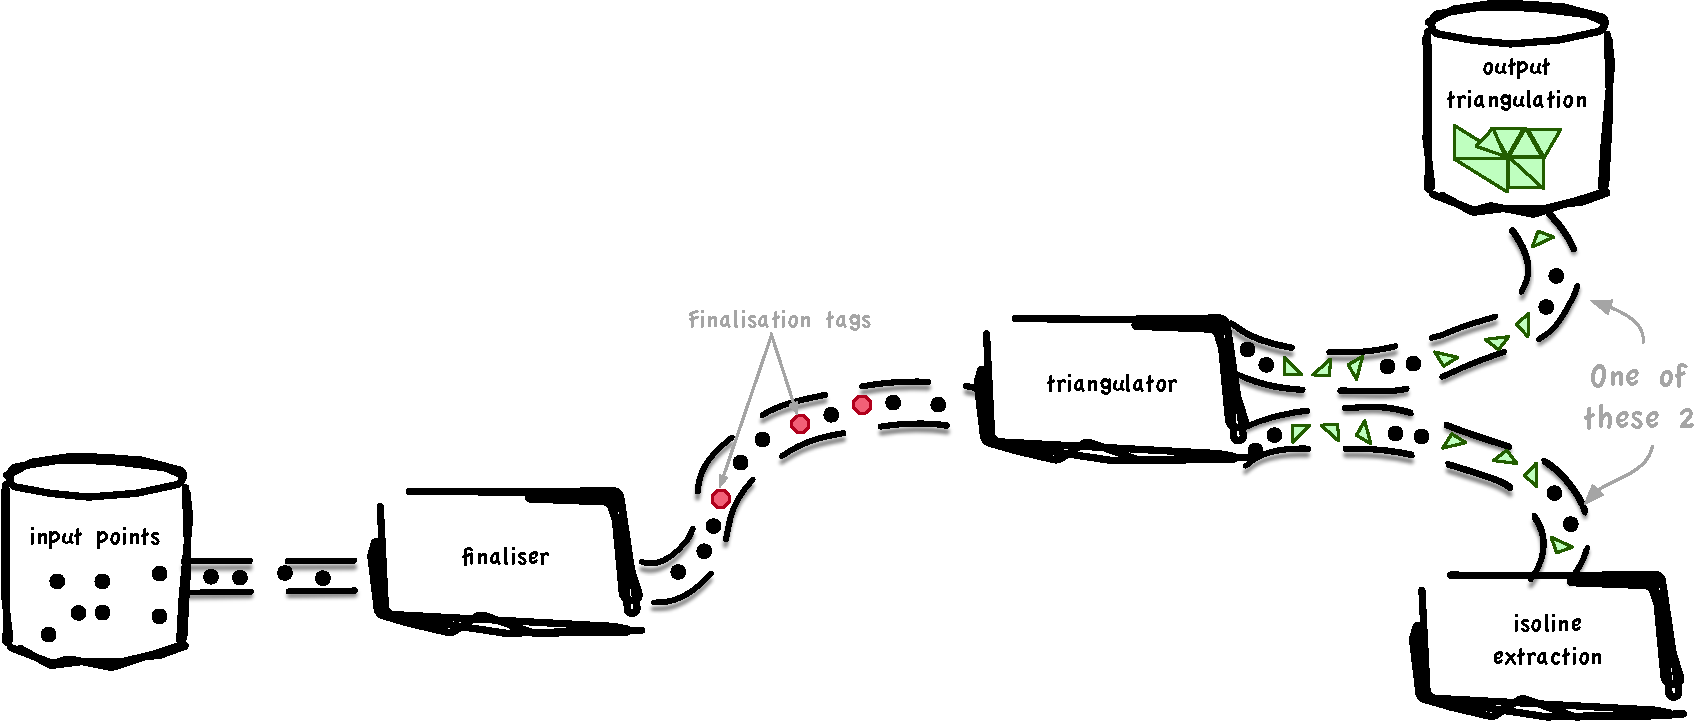
\includegraphics[width=\linewidth]{figs/streaming_pipeline}
  \caption{.}%
\label{fig:streamingdt}
\end{figure}

%%%
\paragraph{Finaliser: adding finalisation tags.}
The key idea is to \emph{preprocess} a set $S$ of points and insert \emph{finalisation tags} informing that certain points/areas will not be needed again.
For the DT construction, as shown in Figure~\ref{fig:finaliser}, this can be realised by constructing a quadtree of $S$; a finalisation tag basically informs the following processes that a certain cell of the quadtree is empty, that all the points have been processed.
\begin{figure*}
  \centering
  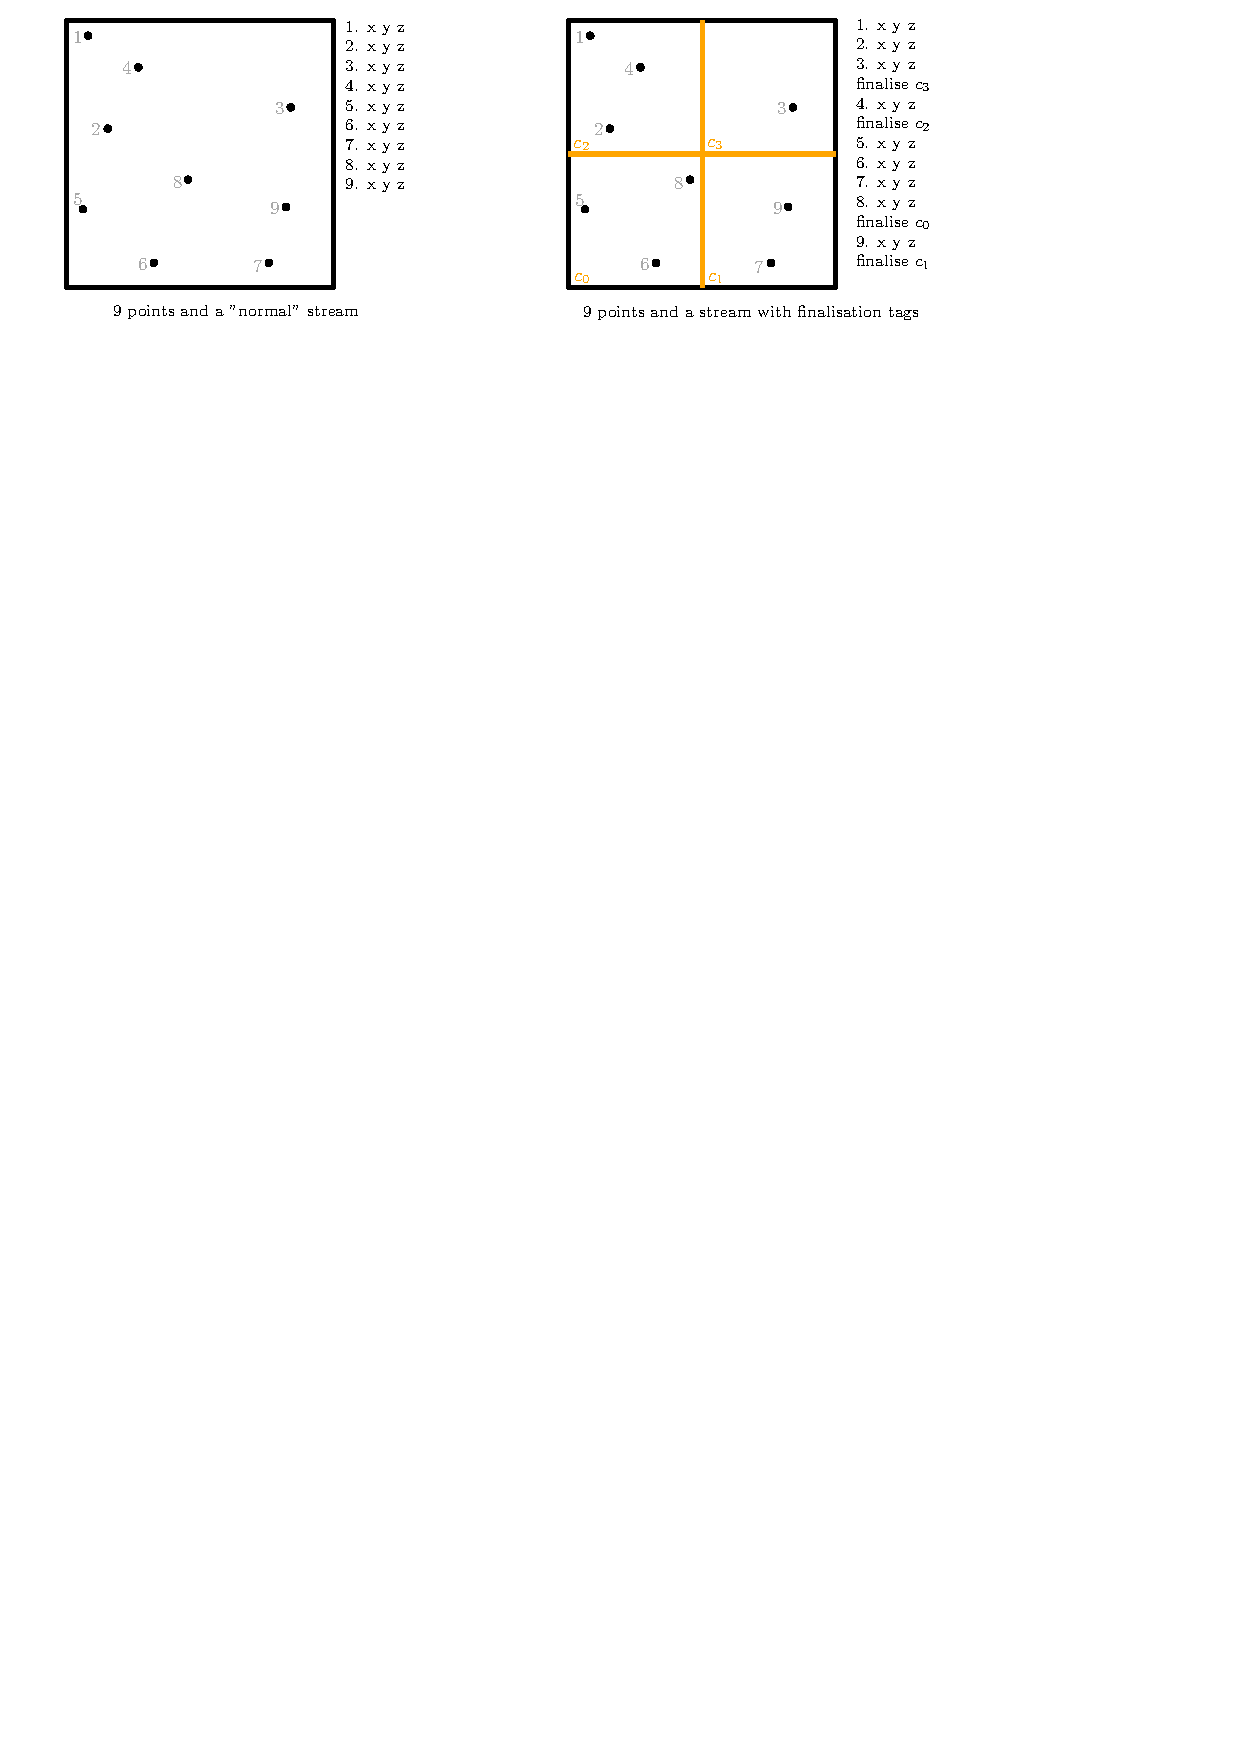
\includegraphics[width=\linewidth]{figs/finaliser}
  \caption{How the finaliser modifies to input and injects finalisation tags. \textbf{Left:} 9 points and the related streams (just a list of the points with coordinates). \textbf{Right:} if a quadtree of depth 1 (in orange) is used (with 4 cells), then the stream would be augmented with finalisation tags.}%
\label{fig:finaliser}
\end{figure*}


%%%
\paragraph{Triangulator.}
The input of the triangulator is the output of the finaliser: a set of points with finalisation tags.
The triangulator will triangulate the points as described in Section~\ref{sec:dtconstruction}, but will attempt to remove memory the triangles that are \emph{final}, those that we are sure will never be modified (since it it guaranteed that no new points will fall inside their circumcircle).
This is performed with the finalisation tags and the following observation (see Figure~\ref{fig:triangulator}): 
\begin{figure}
  \centering
  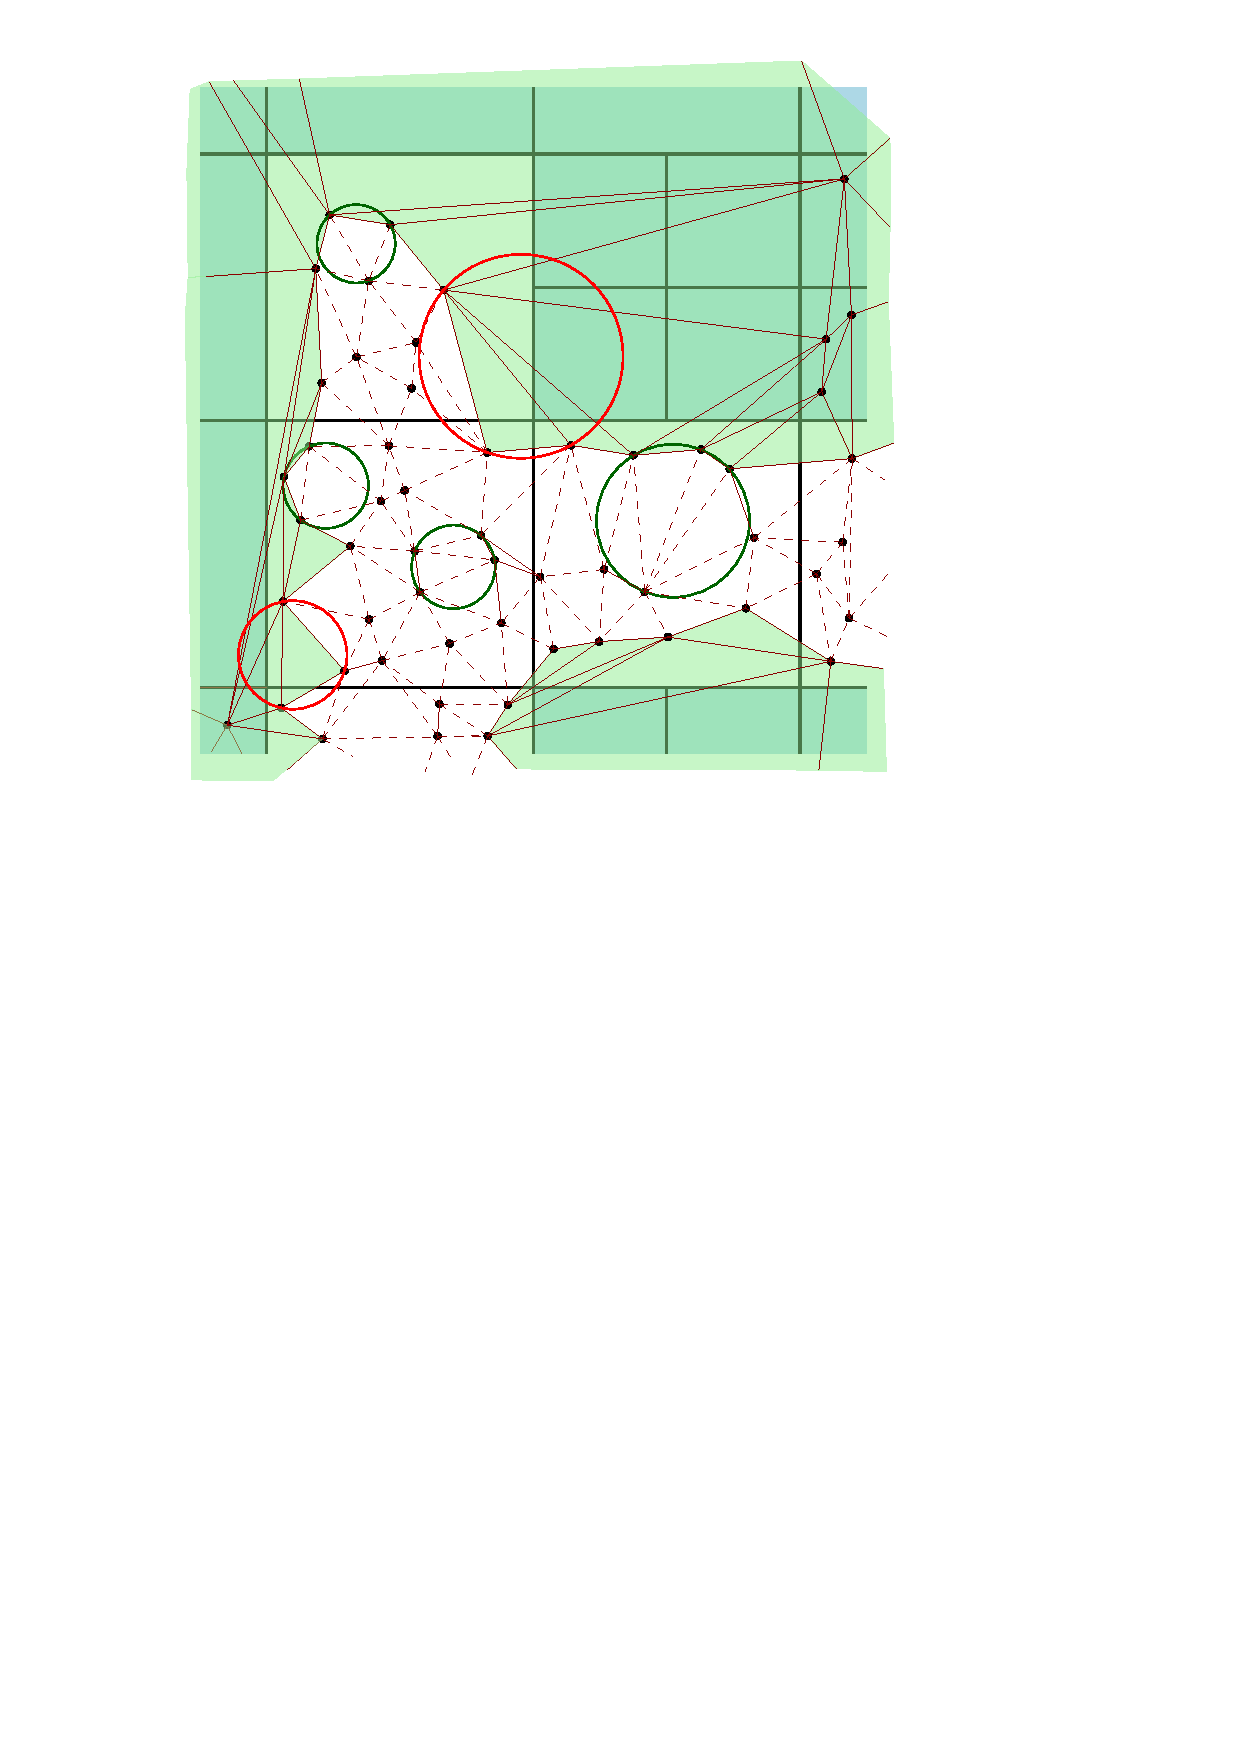
\includegraphics[width=\linewidth]{figs/triangulator}
  \caption{The DT at a given moment during the triangulation process. Blue quadtree cells are not finalised yet, white ones are; green triangles are still in memory (their circumcircle (red circles) encroach on unfinalised cells); white triangles have been written to disk since their circumcircle does not encroach on an active cell (some green circles shown as example).}%
\label{fig:triangulator}
\end{figure}
a triangle inside a finalised quadtree cell (\ie\ where all the points in the streams inside that cell have been read) is final if its circumcircle does not encroach on an active quadtree cell.
If its circumcircle overlaps with an active quadtree cell, then it is possible that further in the stream a new point will be added inside the circle and thus the triangle will not be Delaunay.
Final triangles can be removed from memory and written to disk; it is also possible to add another process to the pipeline and send the final triangles to them.

% TODO: how many are kept in memory? or only in the video?


%%%
\paragraph{Spatial coherence.} % TODO: finish spatial coherence

The constuction of a DT with the streaming paradigm will only work (in the sense that the memory footprint will stay relatively low) if the \emph{spatial coherence}%
\index{spatial coherence}\marginnote{spatial coherence} 
of the input dataset is high.
It is defined by \sidecitet{Isenburg06} as: ``a correlation between the proximity in space of geometric entities and the proximity of their representations in [the file]''.
They demonstrate that real-world point cloud datasets often have natural spatial coherence because the points are usually stored in the order they were collected.
If we shuffled randomly the points in an input file, then the spatial coherence would be very low and the finalisation tags in the stream coming out of the finaliser would be located at the end (and now distributed in the stream).

Figure~\ref{fig:spatial_coherence}
\begin{figure*}
  \centering
  \begin{subfigure}[b]{0.45\linewidth}
    \centering
    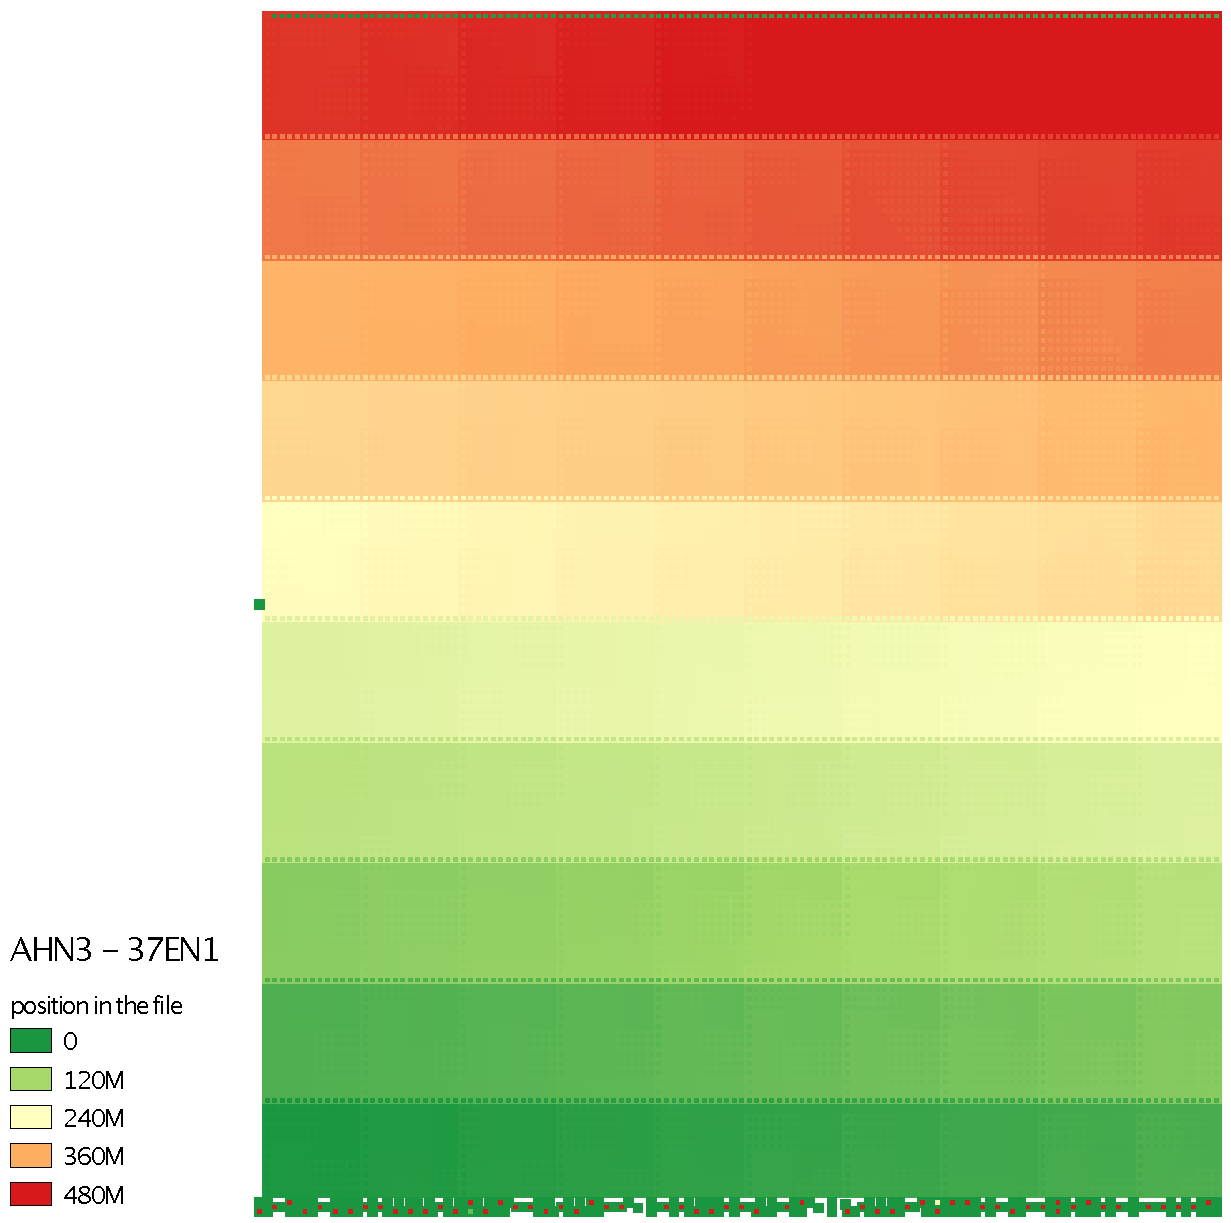
\includegraphics[width=\textwidth]{figs/37EN1_double}
    \caption{}
  \end{subfigure}%
  \qquad
  \begin{subfigure}[b]{0.45\linewidth}
    \centering
    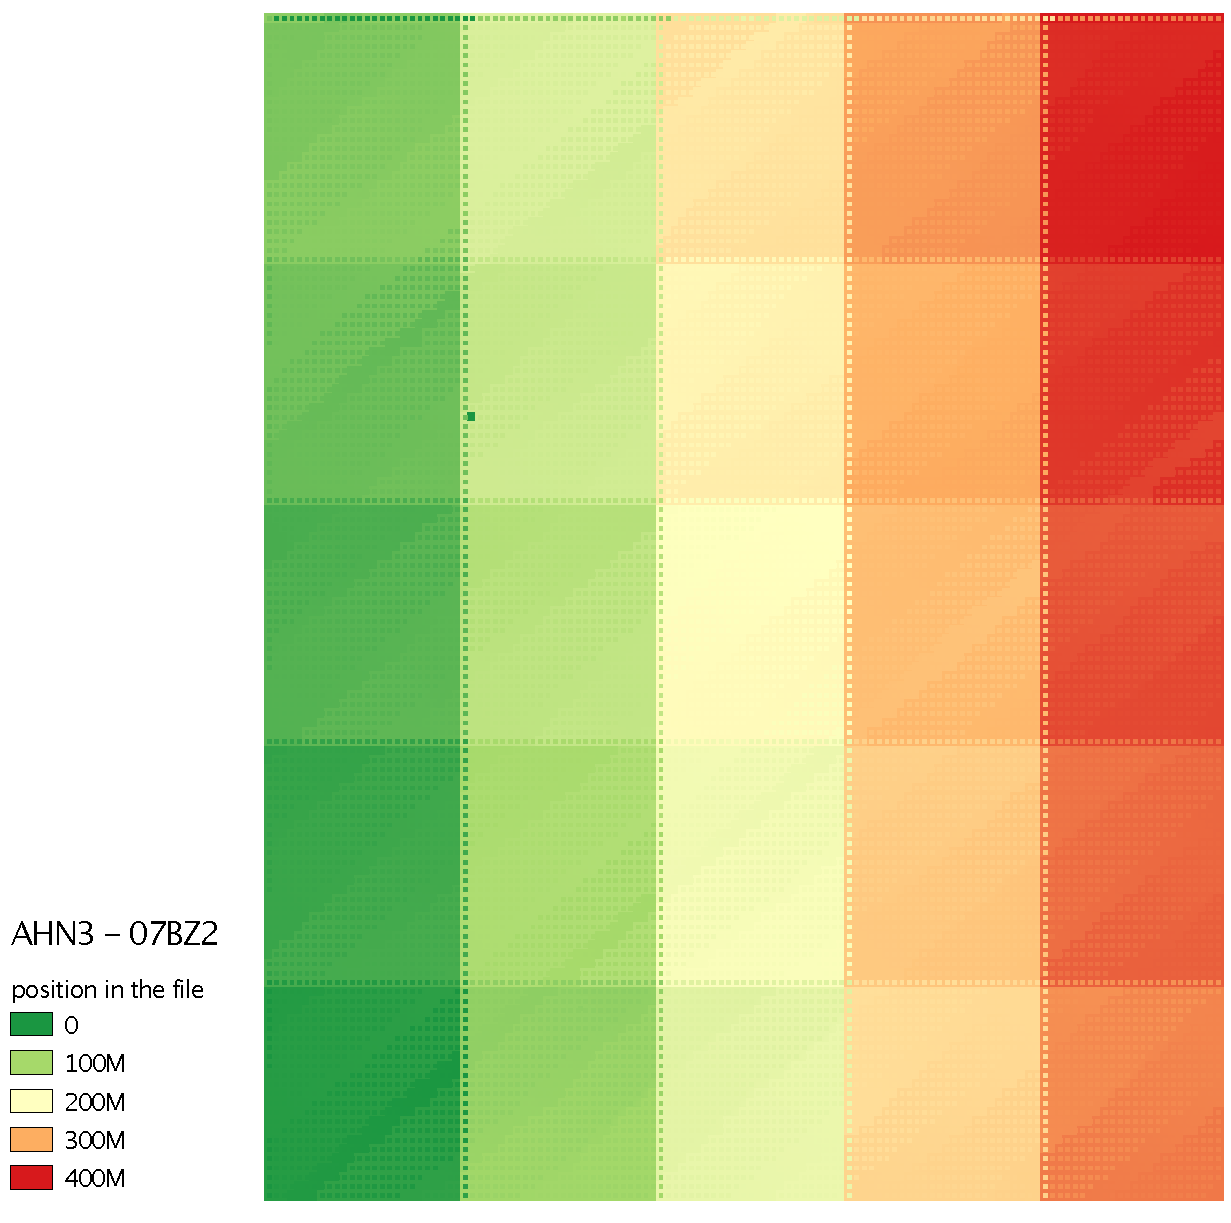
\includegraphics[width=\textwidth]{figs/07BZ2-double}
    \caption{}
  \end{subfigure}
\caption{Spatial coherence of 2 AHN3 tiles. The inner cell colour indicates the position in the stream of first point in that cell, and the outer cell colour indicates the position in the stream of the last point in that cell.}%
\label{fig:spatial_coherence}
\end{figure*}
illustrates the spatial coherence for 2 tiles of the AHN3 dataset\marginnote{\url{https://www.ahn.nl/}} in the Netherlands.
Notice that the cells are generally of the same colour, which means that the spatial coherence is relatively high.
The two datasets are different patterns probably because they were compiled by different companies, who used different equipment and processing software to generate the datasets.


% TODO: streaming useful for other ops?
%%%
\paragraph{What problems.}
The ideas behind streaming are very useful for certain \emph{local} problems (\eg\ interpolation and creation of grids), but unfortunately they cannot be used directly (or it would be extremely challenging) for \emph{global} problems such as visibility or flow modelling.

\begin{kaobox-toread}[frametitle=\faExternalLink\ To read or to watch]
  This video explains how the streaming concepts can be applied to constructing the Delaunay triangulation of massive datasets.
  You do \underline{not} need to read the full paper, which is \citet{Isenburg06}.
  \\ \\
  \url{https://youtu.be/DRCGTF2y_tM}
\end{kaobox-toread}

\begin{kaobox-toread}[frametitle=\faExternalLink\ To read or to watch]
  \fullcite{Isenburg06-1}
  \\ \\
  PDF: \url{http://dx.doi.org/10.1007/11863939_13}
  \\ \\
  The article summarises \citet{Isenburg06} (you do not need to read it), and shows how large rasters can be constructed with spatial interpolation.
\end{kaobox-toread}


% Notice that the pipeline shown in Figure 6 will work only if the input dataset has enough spatial coherence. Isenburg and Lindstrom (2005) define the maximum number of non-finalized points at any time as the width of a stream, the smaller it is the better the spatial coherence is (the smaller the memory footprint of the application is too); I report in the next section on the width of the datasets used for experiments.

%%%%%%%%%%%%%%%%%%%%
%
\section{Notes \& comments}

The description of the $k$d-tree and the nearest neighbour query is adapted from Wikipedia (\url{https://en.wikipedia.org/wiki/K-d_tree}) and the lecture notes entitled ``kd-Trees---CMSC 420'' from Carl Kingsford (available at \url{https://www.cs.cmu.edu/~ckingsf/bioinfo-lectures/kdtrees.pdf}).

\citet{Vitter01} provides an overview of external algorithms.


%%%%%%%%%%%%%%%%%%%%
%
\section{Exercises}

\begin{enumerate}
  \item The tree in \reffig{fig:kdtree2} is balanced, but if ($1,3$) had been selected as the root, how would the tree look like?
  \item \citet{Isenburg06-1} argues that real-world point cloud datasets often have natural spatial coherence. Explain why that is the case for lidar datasets.
  \item How to construct a $k$d-tree that is as balanced as possible?
  \item ``The ideas behind streaming are very useful for certain \emph{local} problems, but unfortunately they cannot be used directly for \emph{global} problems such as visibility or flow modelling''. Explain why that is with a concrete example.
\end{enumerate}
